\documentclass[17pt, a0paper, portrait]{tikzposter}

\usepackage{anyfontsize}
\usepackage{fontspec}
\usepackage{qrcode}
\usepackage{amsmath}
\usepackage{tikz-dependency}

\setmainfont{Topic}[
    Path = ./topic-font/,
    Extension = .ttf,
    BoldFont = *-Bold,
]

\setsansfont{Topic}[
    Path = ./topic-font/,
    Extension = .ttf,
    BoldFont = *-Bold,
]

\newcommand{\tabhead}[1]{\textsf{\textbf{#1}}}
\newcommand{\tabheadtight}[1]{%
  {\addfontfeatures{LetterSpace=-3}\tabhead{#1}}%
}
\newcommand{\tabkicker}[1]{%
  {\fontsize{32}{38}\selectfont\textcolor{tabred}{\tabhead{\uppercase{#1}}}}\\[2mm]%
}
\newcommand{\tabkickerL}[1]{%
  {\fontsize{44}{50}\selectfont\textcolor{tabred}{\tabhead{\uppercase{#1}}}}\\[2mm]%
}

% A tight horizontal line that fills the block width.
\newcommand{\tablineTightH}[2]{%
  {\fontsize{#1}{#1}\selectfont\tabheadtight{#2}}%
}

% A tight vertical stack of big text.
\newcommand{\tablineTightV}[2]{%
  \parbox{\linewidth}{\raggedright\fontsize{#1}{#1}\selectfont\tabheadtight{#2}}%
}

\definecolor{tabred}{HTML}{cc0000}
\definecolor{tabink}{HTML}{111111}
\definecolor{tabgrey}{HTML}{e5e5e5}
\definecolor{tabmute}{HTML}{666666}

\colorlet{backgroundcolor}{white}
\colorlet{framecolor}{white}

\definetitlestyle{tabnone}{
    width=0pt, roundedcorners=0, linewidth=0pt, innersep=0pt,
    titletotopverticalspace=0pt, titletoblockverticalspace=0pt,
    titlegraphictotitledistance=0pt, titletextscale=0.001
}{}
\usetitlestyle{tabnone}
\colorlet{titlefgcolor}{tabink}
\colorlet{titlebgcolor}{white}

\defineblockstyle{tabloid}{titlewidthscale=1, bodywidthscale=1,
        titleleft, titleoffsetx=0pt, titleoffsety=0pt,
        bodyoffsetx=0pt, bodyoffsety=0pt,
        bodyverticalshift=2mm, roundedcorners=0,
        linewidth=0pt, titleinnersep=2pt, bodyinnersep=6pt}{
    \ifBlockHasTitle
        \draw[draw=tabink, line width=6pt]
            (blocktitle.south west) -- (blocktitle.south east);
    \fi
}
\useblockstyle{tabloid}

\defineblockstyle{masthead}{titlewidthscale=1, bodywidthscale=1,
        titleleft, titleoffsetx=0pt, titleoffsety=0pt,
        bodyoffsetx=0pt, bodyoffsety=0pt,
        bodyverticalshift=0mm, roundedcorners=0,
        linewidth=0pt, titleinnersep=0pt, bodyinnersep=0pt}{}

\defineblockstyle{tabgrey}{titlewidthscale=1, bodywidthscale=1,
        titleleft, titleoffsetx=0pt, titleoffsety=0pt,
        bodyoffsetx=0pt, bodyoffsety=0pt,
        bodyverticalshift=2mm, roundedcorners=0,
        linewidth=0pt, titleinnersep=4pt, bodyinnersep=14pt}{
    \draw[fill=tabgrey, draw=tabgrey]
        (blockbody.south west) rectangle (blocktitle.north east);
    \ifBlockHasTitle
        \draw[draw=tabink, line width=6pt]
            (blocktitle.south west) -- (blocktitle.south east);
    \fi
}

\colorlet{blocktitlebgcolor}{white}
\colorlet{blocktitlefgcolor}{tabink}
\colorlet{blockbodybgcolor}{white}
\colorlet{blockbodyfgcolor}{tabink}

\begin{document}

\title{}
\author{}
\maketitle

\useblockstyle{masthead}
\block{}{
  \vspace{-2cm}
  % --- Dateline bar.
  \rule{\linewidth}{2pt}\\[2mm]
  \makebox[\linewidth]{%
    {\fontsize{42}{48}\selectfont\tabhead{May 16, 2026}}\hfill
    {\fontsize{38}{44}\selectfont Universal Dependencies Workshop \;\textbar\; LREC 2026 \;\textbar\; Vol.~26 \;\textbar\; Exclusive}}\\[2mm]
  \rule{\linewidth}{2pt}\\[10mm]

  % --- RED KICKER, all caps, left-aligned. Conspiratorial parody.
  {\fontsize{96}{104}\selectfont\tabhead{\textcolor{tabred}{BIG SYNTAX DOESN'T WANT YOU TO KNOW}}}\\[6mm]

  % --- HEADLINE: edge-to-edge giant tabloid scream, with tight word spacing.
  \tablineTightH{340pt}{MAL is universal? Hardly.}\\[-25mm]
  \rule{\linewidth}{30pt}\\[10mm]

  % --- Sub-deck + authors + QR in one horizontal band
  \begin{minipage}[c]{0.82\linewidth}
    \tablineTightH{96pt}{The Menzerath-Altmann law on all 180 UD treebanks}\par\vspace{8mm}
    \begin{center}
    {\fontsize{38}{44}\selectfont\textbf{%
      Pegah Faghiri\textsuperscript{1,2} \quad
      Kim Gerdes\textsuperscript{2} \quad
      Sylvain Kahane\textsuperscript{1,3}}}\\[4mm]
    {\fontsize{30}{36}\selectfont
      \textsuperscript{1}Modyco, CNRS \& Paris Nanterre University \quad
      \textsuperscript{2}LISN, CNRS \& Paris-Saclay University \quad
      \textsuperscript{3}Institut Universitaire de France}
    \end{center}
  \end{minipage}\hfill
  \begin{minipage}[c]{0.16\linewidth}\centering
    \qrcode[height=6cm, level=H]{https://typometrics.elizia.net/menzerath}\par\vspace{4mm}
    {\fontsize{30}{34}\selectfont \textbf{typometrics.elizia.net}}\par\vspace{2mm}
    {\Large Interactive maps \& curves}
  \end{minipage}\par\vspace{5mm}
  \rule{\linewidth}{2pt}
}
\useblockstyle{tabloid}

% =====================================================================
% SECTION 1: HOW MAL IS COMPUTED
% =====================================================================
\begin{columns}
\column{0.50}
\useblockstyle{tabgrey}
\block{%
  \tabkicker{How we compute MAL}

  \tablineTightH{70pt}{Real constituents only. Fake dependents eliminated!}}{
  \raggedright
  \vspace{4pt}
  {\huge The \textbf{Menzerath-Altmann law} (MAL) predicts that ``the greater the number of components of a given unit, the shorter their respective length'' (Menzerath, 1928). In the verbal domain: as the number of dependents $n$ grows, their average size decreases.}\par\vspace{5mm}

  {\huge Altmann (1980) formalised this as a \textbf{power law}: $\text{MAL}_n \approx n^{-\beta}$, i.e.\ $\log(\text{MAL}_n) \approx -\beta \cdot \log(n)$. The slope $\beta$ measures the \textbf{MAL effect}. Previous studies: Macutek et al.\ (2017) for Czech; Tanaka-Ishii (2021) for UD~2.3 without filtering.}\par\vspace{5mm}

  {\huge \textbf{NEW!}\ Our data extraction is filtered: we exclude \texttt{punct, discourse, parataxis, conj, cc, vocative, aux, compound:prt, mark, case} from the verbal construction. Only \textbf{real syntactic constituents} are retained.}\par\vspace{5mm}

  {\huge \textbf{What about ``bastards''?} A constituent's subtree may spill across the verb. We count the spilled part as a separate dependent of the verb:}\par\vspace{4mm}

  % --- Dependency tree: 'Vogel' comes from German which means bird
  % UD_English-GUM, GUM_whow_languages-17 — rendered with reactive-dep-tree
  \begin{center}
  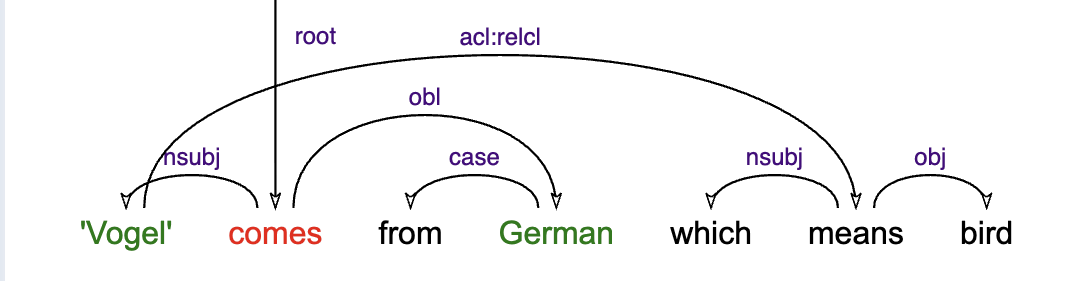
\includegraphics[width=0.85\linewidth]{bastard_tree.png}
  \end{center}
  \vspace{2mm}
  {\huge The relative clause ``which means bird'' (\textbf{acl:relcl}) syntactically depends on `Vogel' (left of verb) but appears right of verb --- a \textbf{bastard}. It is counted as a right-side constituent of \textbf{comes}. Source: \textit{en\_gum}.}\par\vspace{3mm}
}

\column{0.50}
\block{%
  \tabkicker{NEW! Left vs.\ right}

  \tablineTightH{90pt}{Two sides of the verb, two different worlds}}{
  \raggedright
  \vspace{4pt}
  {\huge We compute three variants of the MAL effect:}\par\vspace{8mm}

  \begin{minipage}[t]{0.48\linewidth}
    {\fontsize{44}{50}\selectfont\tabhead{MAL}}\par\vspace{4mm}
    {\huge $\text{MAL}_n(L)$ = mean size of constituents in all verbal constructions of L with $n$ constituents (left + right combined). Standard MAL as in the literature.}
  \end{minipage}\hfill
  \begin{minipage}[t]{0.48\linewidth}
    {\fontsize{44}{50}\selectfont\tabhead{LMAL \& RMAL\quad\textcolor{tabred}{NEW!}}}\par\vspace{4mm}
    {\huge $\text{LMAL}_n(L)$ = mean size of constituents in constructions with $n$ \textbf{preverbal} (left) constituents, regardless of the right side.}\par\vspace{5mm}
    {\huge $\text{RMAL}_n(L)$ = mean size of constituents in constructions with $n$ \textbf{postverbal} (right) constituents, regardless of the left side.}
  \end{minipage}\par\vspace{12mm}

  {\huge \textbf{MAL effect} $= \beta$, the slope of the regression line in log-log space. $\beta > 0.1$: \textbf{MAL language}. $\beta < -0.1$: \textbf{Anti-MAL}. In between: \textbf{grey zone}.}\par\vspace{8mm}

  {\huge \textbf{Why does this matter?} DLM (Dependency Length Minimization) predicts short-before-long postverbally and long-before-short preverbally. Unlike DLM, MAL is direction-free. So: \textbf{does MAL hold equally on both sides?} Spoiler: \textbf{no.}}\par\vspace{3mm}
}
\useblockstyle{tabloid}
\end{columns}

% =====================================================================
% SECTION 2: CASE STUDIES
% =====================================================================
\block{%
  \tabkicker{As usual}

  {\fontsize{78}{86}\selectfont\tabhead{German nails it. Naija wobbles. Arabic surprises. You?}}}{
  \raggedright
  \begin{minipage}[t]{0.31\linewidth}\raggedright
    \vspace{0pt}
    \includegraphics[width=\linewidth]{../plots/German_loglog}\par\vspace{3mm}
    {\fontsize{38}{44}\selectfont\tabhead{German -- textbook MAL}}\par\vspace{3mm}
    {\huge \textbf{slope = --0.17, R\textsuperscript{2} \textasciitilde\ 0.89}
     on the log-log fit. A near-perfect power law: every extra
     dependent shrinks the average constituent. German is MAL,
     RMAL and LMAL as expected. Is anyone surprised?}
  \end{minipage}\hfill
  \begin{minipage}[t]{0.31\linewidth}\raggedright
    \vspace{0pt}
    \includegraphics[width=\linewidth]{../plots/Naija_loglog}\par\vspace{3mm}
    {\fontsize{38}{44}\selectfont\tabhead{Naija -- mixed, asymmetric}}\par\vspace{3mm}
    {\huge Left and right dependents diverge wildly. A young
     pidgincreole refusing to fit one curve --- in fact the
     \textbf{strongest Anti-LMAL in the whole sample}
     ($\beta=+0.73$ preverbally).}
  \end{minipage}\hfill
  \begin{minipage}[t]{0.31\linewidth}\raggedright
    \vspace{0pt}
    \includegraphics[width=\linewidth]{../plots/Arabic_loglog}\par\vspace{3mm}
    {\fontsize{38}{44}\selectfont\tabhead{Arabic -- complex behavior}}\par\vspace{3mm}
    {\huge Arabic has a particularly low R\textsuperscript{2}. It follows MAL from $n=1$ to $3$, but becomes Anti-MAL from $n=3$ onwards.\\[3mm]
    \textbf{And you?} Check your language at \textbf{typometrics.elizia.net}!}
  \end{minipage}\par

  \vspace{4mm}
}

% =====================================================================
% SECTION 3: RESULTS (Bar charts from paper tables)
% =====================================================================
\useblockstyle{tabgrey}
\block{%
  \tabkickerL{The numbers nobody talks about}

  {\fontsize{72}{80}\selectfont\tabhead{MAL is not ambidextrous. The verb leans right.}}}{
  \raggedright
  \begin{minipage}[t]{0.30\linewidth}\raggedright
    \vspace{0pt}
    {\centering\includegraphics[width=\linewidth]{../plots/poster_strip_mal}\par}
    \vspace{3mm}
    {\fontsize{38}{44}\selectfont\tabhead{MAL by word order}}\par\vspace{3mm}
    {\huge MAL is stronger for \textbf{VO languages} (56\%) than OV (42\%), but RMAL and LMAL are \textbf{stronger for OV}! Where does the paradox come from?}
  \end{minipage}\hfill
  \begin{minipage}[t]{0.30\linewidth}\raggedright
    \vspace{0pt}
    {\centering\includegraphics[width=\linewidth]{../plots/poster_strip_rmal}\par}
    \vspace{3mm}
    {\fontsize{38}{44}\selectfont\tabhead{RMAL: postverbal domain}}\par\vspace{3mm}
    {\huge \textbf{79\% of UD languages are RMAL} (81/103) and only \textbf{7\% are Anti-RMAL} (7/103). The right side of the verb strongly compresses constituent size as $n$ grows. VO languages lead: 84\% are RMAL vs.\ 63\% for OV.}
  \end{minipage}\hfill
  \begin{minipage}[t]{0.30\linewidth}\raggedright
    \vspace{0pt}
    {\centering\includegraphics[width=\linewidth]{../plots/poster_strip_lmal}\par}
    \vspace{3mm}
    {\fontsize{38}{44}\selectfont\tabhead{LMAL: preverbal domain}}\par\vspace{3mm}
    {\huge Only \textbf{31\% are LMAL} (39/124) and \textbf{23\% are Anti-LMAL} (29/124). The left side of the verb resists compression --- or even reverses it. OV languages are better: 39\% are LMAL vs.\ 29\% for VO. VO languages are \textbf{3$\times$} more likely to be Anti-LMAL.}
  \end{minipage}\par
  \vspace{4mm}
}
\useblockstyle{tabloid}

% =====================================================================
% CALL TO ACTION - compact footer
% =====================================================================
\block{%
  \tabkicker{It's 100\% free*}
  {\fontsize{62}{70}\selectfont\tabhead{Come and find out how your UD language is doing!}}}{
  \raggedright
  {\huge \textbf{180 treebanks}, interactive PCA + family map +
    per-language curves + compliance ridgeline --- all at \textbf{typometrics.elizia.net/menzerath}.
    \textcolor{tabmute}{*~\itshape Free as in
    beer, free as in speech, free as in dependency.}}
}

\end{document}
